
\subsection{UC-1 Registrazione}

\begin{figure}[H]
	\centering
	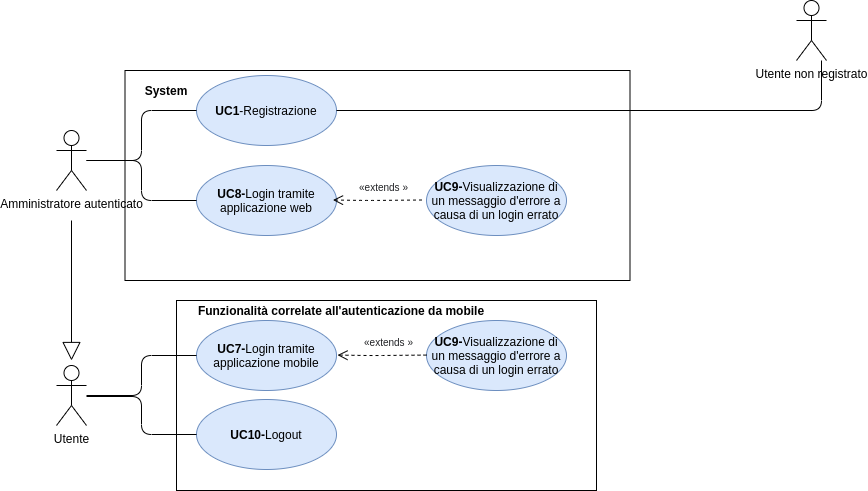
\includegraphics[width=\textwidth]{src/CasiDUso/immagini/Autenticazione.png}
	\caption{UC-1,7,8,9,10.}
\end{figure}

\begin{itemize}
	\item \textbf{Attore primario:} amministratore autenticato;

	\item \textbf{Attori secondari}: utente;

	\item \textbf{Descrizione:} l'amministratore vuole registrare un nuovo utente presso il sistema tramite indirizzo e-mail e password. Viene richiesto anche l'inserimento del nome e del cognome del nuovo utente. All'utente non registrato viene richiesto l'inserimento di una password personale;

	\item \textbf{Precondizioni:} l'utente non possiede un account, pertanto non è registrato all'interno del sistema. L'amministratore è autenticato presso il sistema;

	\item \textbf{Postcondizioni:} l'utente è censito all'interno del sistema;

	\item \textbf{Scenario principale:}
	      \begin{enumerate}
		      \item l'amministratore seleziona la funzionalità di inserimento di un nuovo utente;
		      \item l'amministratore inserisce il nome dell'utente da registrare (UC-1.1 inserimento del nome di un nuovo utente non registrato);
		      \item l'amministratore inserisce il cognome dell'utente da registrare(UC-1.2 inserimento del cognome di un nuovo utente non registrato);
		      \item l'amministratore inserisce l'indirizzo e-mail con il quale il nuovo utente si autenticherà presso il sistema(UC-1.3 inserimento dell'indirizzo e-mail di un nuovo utente non registrato);
		      \item l'amministratore invia i dati inseriti al sistema il quale invia, all'indirizzo e-mail precedentemente inserito, un link attraverso terminare la registrazione(UC-4 Creazione di una nuova password personale).
	      \end{enumerate}
\end{itemize}

\begin{figure}[H]
	\centering
	  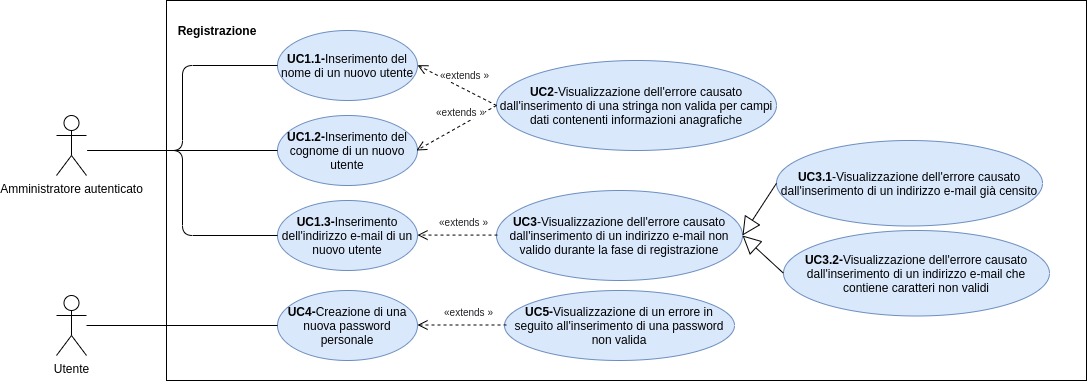
\includegraphics[width=\textwidth]{src/CasiDUso/immagini/SottocasiRegistrazione.png}
	\caption{Zoom-in registrazione.}
  \end{figure}

\subsection{UC-1.1 Inserimento del nome di un nuovo utente}
\begin{itemize}
	\item \textbf{Attore primario:} amministratore autenticato;

	\item \textbf{Descrizione:} l'amministratore vuole inserire il nome di un utente che deve essere registrato presso il sistema;

	\item \textbf{Precondizioni:} l'amministratore è autenticato presso il sistema e ha selezionato la funzionalità di inserimento di un nuovo utente non registrato;

	\item \textbf{Postcondizioni:} l'amministratore ha inserito con successo il nome dell'utente da registrare;

	\item \textbf{Scenario principale:}
	      \begin{enumerate}
		      \item l'amministratore seleziona il campo dati in cui inserire il nome dell'utente da registrare;
		      \item l'amministratore inserisce il nome dell'utente da registrare.
	      \end{enumerate}
	\item \textbf{Estensioni:}
	      \begin{enumerate}
		      \item UC-2 Visualizzazione dell'errore causato dall'inserimento di una stringa non valida per campi dati contenenti informazioni anagrafiche.
	      \end{enumerate}
\end{itemize}
\subsection{UC-1.2 Inserimento del cognome di un nuovo utente}
\begin{itemize}
	\item \textbf{Attore primario:} amministratore autenticato;

	\item \textbf{Descrizione:} l'amministratore vuole inserire il cognome di un utente che deve essere registrato presso il sistema;

	\item \textbf{Precondizioni:} l'amministratore è autenticato presso il sistema e ha selezionato la funzionalità di inserimento di un nuovo utente non registrato;

	\item \textbf{Postcondizioni:} l'amministratore ha inserito con successo il cognome dell'utente da registrare;

	\item \textbf{Scenario principale:}
	      \begin{enumerate}
		      \item l'amministratore seleziona il campo dati in cui inserire il cognome dell'utente da registrare;
		      \item l'amministratore inserisce il cognome dell'utente da registrare.
	      \end{enumerate}
	\item \textbf{Estensioni:}
	      \begin{enumerate}
		      \item UC-2 Visualizzazione dell'errore causato dall'inserimento di una stringa non valida per campi dati contenenti informazioni anagrafiche.
	      \end{enumerate}
\end{itemize}
\subsection{UC-1.3 Inserimento dell'indirizzo e-mail di un nuovo utente}
\begin{itemize}
	\item \textbf{Attore primario:} amministratore autenticato;

	\item \textbf{Descrizione:} l'amministratore vuole inserire l'indirizzo e-mail di un utente che deve essere registrato presso il sistema;

	\item \textbf{Precondizioni:} l'amministratore è autenticato presso il sistema e ha selezionato la funzionalità di inserimento di un nuovo utente non registrato;

	\item \textbf{Postcondizioni:} l'amministratore ha inserito con successo l'indirizzo e-mail dell'utente da registrare;

	\item \textbf{Scenario principale:}
	      \begin{enumerate}
		      \item l'amministratore seleziona il campo dati in cui inserire l'indirizzo e-mail dell'utente da registrare;
		      \item l'amministratore inserisce l'indirizzo e-mail dell'utente da registrare.
	      \end{enumerate}

	\item \textbf{Estensioni:}
	      \begin{enumerate}
		      \item UC-3Visualizzazione dell'errore causato dall'inserimento di un indirizzo e-mail non valido durante la fase di registrazione.
	      \end{enumerate}
\end{itemize}
\subsection{UC-2 Visualizzazione dell'errore causato dall'inserimento di una stringa non valida per campi dati contenenti informazioni anagrafiche.}
\begin{itemize}
	\item \textbf{Attore primario:} amministratore autenticato;

	\item \textbf{Descrizione:} l'amministratore ha provato a registrare un nuovo utente ma la registrazione non è andata a buon fine poiché uno o entrambi i dati anagrafici(nome,cognome) inseriti non risultavano validi(es.ci sono numeri o caratteri speciali);

	\item \textbf{Precondizioni:} l'amministratore ha inserito almeno un dato anagrafico non valido durante la registrazione e ha inviato i dati al sistema;

	\item \textbf{Postcondizioni:} il sistema restituisce un messaggio d'errore esplicativo e non completa la registrazione del nuovo utente;

	\item \textbf{Scenario principale:}
	      \begin{enumerate}
		      \item il sistema elabora la richiesta ricevuta;
		      \item il sistema restituisce un messaggio d'errore esplicativo che viene visualizzato sullo schermo del dispositivo dell'amministratore e non completa la registrazione del nuovo utente.
	      \end{enumerate}
\end{itemize}

\subsection{UC-3 Visualizzazione dell'errore causato dall'inserimento di un indirizzo e-mail non valido durante la fase di registrazione}
\begin{itemize}
	\item \textbf{Attore primario:} amministratore autenticato;

	\item \textbf{Descrizione:} l'amministratore ha provato a registrare un nuovo utente ma la registrazione non è andata a buon fine poiché l'indirizzo e-mail risultava già censito(UC-3.1) o inadeguato ai criteri stabiliti per la creazione di un indirizzo e-mail(UC-3.2);

	\item \textbf{Precondizioni:} l'amministratore ha inserito un indirizzo e-mail non valido durante la registrazione e ha inviato i dati al sistema;

	\item \textbf{Postcondizioni:} il sistema restituisce un messaggio d'errore esplicativo e non completa la registrazione del nuovo utente;

	\item \textbf{Scenario principale:}
	      \begin{enumerate}
		      \item il sistema elabora la richiesta ricevuta;
		      \item il sistema restituisce un messaggio d'errore esplicativo che viene visualizzato sullo schermo del dispositivo dell'amministratore e non completa la registrazione del nuovo utente.
	      \end{enumerate}
\end{itemize}

\subsubsection{UC-3.1 Visualizzazione dell'errore causato dall'inserimento di un indirizzo e-mail già censito}
\begin{itemize}
	\item \textbf{Attore primario:} amministratore autenticato;

	\item \textbf{Descrizione:} l'amministratore ha provato a registrare un nuovo utente ma la registrazione non è andata a buon fine poiché l'indirizzo e-mail inserito è già associato ad un altro utente all'interno del sistema;

	\item \textbf{Precondizioni:} l'amministratore ha inserito un indirizzo e-mail già utilizzato da un altro utente durante la registrazione e ha inviato i dati al sistema;

	\item \textbf{Postcondizioni:} il sistema restituisce un messaggio d'errore esplicativo e non completa la registrazione del nuovo utente;

	\item \textbf{Scenario principale:}
	      \begin{enumerate}
		      \item il sistema elabora la richiesta ricevuta;
		      \item il sistema restituisce un messaggio d'errore esplicativo che viene visualizzato sullo schermo del dispositivo dell'amministratore e non completa la registrazione del nuovo utente.
	      \end{enumerate}
\end{itemize}
\subsubsection{UC-3.2 Visualizzazione dell'errore causato dall'inserimento di un indirizzo e-mail che contiene caratteri non validi}
\begin{itemize}
	\item \textbf{Attore primario:} amministratore autenticato;

	\item \textbf{Descrizione:} l'amministratore ha provato a registrare un nuovo utente ma la registrazione non è andata a buon fine poiché l'indirizzo e-mail inserito contiene dei caratteri speciali che non rispettano i criteri di inserimento di un nuovo indirizzo e-mail;

	\item \textbf{Precondizioni:} l'amministratore ha inserito un indirizzo e-mail che contiene dei caratteri non validi durante la registrazione e ha inviato i dati al sistema;

	\item \textbf{Postcondizioni:} il sistema restituisce un messaggio d'errore esplicativo e non completa la registrazione del nuovo utente;

	\item \textbf{Scenario principale:}
	      \begin{enumerate}
		      \item il sistema elabora la richiesta ricevuta;
		      \item il sistema restituisce un messaggio d'errore esplicativo che viene visualizzato sullo schermo del dispositivo dell'amministratore e non completa la registrazione del nuovo utente.
	      \end{enumerate}
\end{itemize}

\subsection{UC-4 Creazione di una nuova password personale}
\begin{itemize}
	\item \textbf{Attore primario:} utente (non registrato/registrato/autenticato/non autenticato);

	\item \textbf{Descrizione:} l'utente vuole inserire una nuova password;

	\item \textbf{Precondizioni:} l'utente ha cliccato il link per l'impostazione di una nuova password ricevuto via indirizzo e-mail;

	\item \textbf{Postcondizioni:} l'utente ha cambiato la propria password con successo;

	\item \textbf{Scenario principale:}
	      \begin{enumerate}
		      \item l'utente inserisce la nuova password all'interno del campo dati della pagina aperta tramite link;
		      \item l'utente conferma con successo la password inserita (UC-4.1 Conferma della password inserita);
		      \item il sistema restituisce un messaggio comunicante l'avvenuto cambiamento della password.
	      \end{enumerate}

	      \textbf{Estensioni:}
	      \begin{enumerate}
		      \item UC-5Visualizzazione di un errore in seguito all'inserimento di una password non valida;
	      \end{enumerate}
\end{itemize}

\begin{figure}[H]
	\centering
	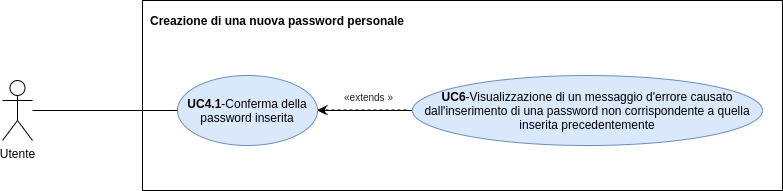
\includegraphics[width=\textwidth]{src/CasiDUso/immagini/SottocasoCreazionePassword.png}
	\caption{Zoom-in creazione password.}
\end{figure}

\subsubsection{UC-4.1 Conferma della password inserita}
\begin{itemize}
	\item \textbf{Attore primario:} utente;

	\item \textbf{Descrizione:} l'utente vuole confermare la password inserita;

	\item \textbf{Precondizioni:} l'utente ha inserito una nuova password valida all'interno della pagina per l'inserimento di una nuova password;

	\item \textbf{Postcondizioni:} l'utente ha inserito con successo la stessa password inserita precedentemente;

	\item \textbf{Scenario principale:}
	      \begin{enumerate}
		      \item l'utente inserisce la password precedentemente inserita;
		      \item il sistema analizza il matching tra le due password e in caso di errore restituisce un messaggio d'errore esplicativo e richiede nuovamente l'inserimento di una nuova password senza precedentemente completare la modifica della password.
	      \end{enumerate}
	\item \textbf{Estensioni:}
	      \begin{enumerate}
		      \item UC-6 Visualizzazione di un messaggio d'errore causato dall'inserimento di una password non corrispondente a quella inserita precedentemente.
	      \end{enumerate}
\end{itemize}
\subsection{UC-5 Visualizzazione di un errore in seguito all'inserimento di una password non valida}
\begin{itemize}
	\item \textbf{Attore primario:} utente;

	\item \textbf{Descrizione:} viene visualizzato un messaggio d'errore a seguito dell'inserimento di una password non valida da parte di un utente durante l'impostazione di una nuova password;

	\item \textbf{Precondizioni:} l'utente ha inserito una password non valida durante l'impostazione di una nuova password.

	\item \textbf{Postcondizioni:} il sistema restituisce un messaggio d'errore esplicativo e chiede all'utente di inserire una nuova password valida senza apportare le modifiche;

	\item \textbf{Scenario principale:}
	      \begin{enumerate}
		      \item il sistema elabora la richiesta ricevuta;
		      \item il sistema restituisce un messaggio d'errore esplicativo che viene visualizzato sullo schermo del dispositivo dell'utente e non completa la registrazione del nuovo dipendente fino a quando non viene inserita una password corretta.
	      \end{enumerate}
\end{itemize}
\subsection{UC-6 Visualizzazione di un messaggio d'errore causato dall'inserimento di una password non corrispondente a quella inserita precedentemente}
\begin{itemize}
	\item \textbf{Attore primario:} utente;

	\item\textbf{Descrizione:} l'utente vuole confermare la password inserita.Viene visualizzato un messaggio d'errore causato dall'inserimento di una password di conferma errata;

	\item\textbf{Precondizioni:} l'utente ha inserito una nuova password valida all'interno della pagina per l'inserimento di una nuova password e ha inserito una password di conferma diversa da quella inserita precedentemente;

	\item\textbf{Postcondizioni:} viene visualizzato un messaggio d'errore causato dall'inserimento di una password di conferma errata;

	\item \textbf{Scenario principale:}
	      \begin{enumerate}
		      \item l'utente inserisce la password precedentemente inserita;
		      \item il sistema analizza il matching tra le due password e in caso di errore restituisce un messaggio d'errore esplicativo e richiede nuovamente l'inserimento di una nuova password senza precedentemente completare la modifica della password.
	      \end{enumerate}
\end{itemize}
\subsection{UC-7 Login tramite applicazione mobile}
\begin{itemize}
	\item \textbf{Attore primario:} utente registrato;

	\item \textbf{Descrizione:} l'utente vuole autenticarsi presso il sistema tramite l'inserimento del proprio indirizzo e-mail di registrazione e la propria password;

	\item \textbf{Precondizioni:} l'utente è registrato presso il sistema;

	\item \textbf{Postcondizioni:} l'utente è autenticato presso il sistema;

	\item\textbf{Scenario principale:}

	      \begin{enumerate}
		      \item l'utente avvia l'applicazione mobile;
		      \item l'utente seleziona la funzionalità "Accedi";
		      \item l'utente inserisce il proprio indirizzo e-mail con il quale si è registrato presso il sistema;
		      \item l'utente inserisce la propria password;
		      \item l'utente invia i dati al sistema;
		      \item Il sistema elabora la richiesta e aggiorna la schermata del dispositivo con la dashboard personale qualora il login venga eseguito con successo. In caso contrario il sistema restituisce un messaggio d'errore esplicativo e non completa il login dell'utente.
	      \end{enumerate}
	\item \textbf{Estensioni:}
	      \begin{enumerate}
		      \item UC-Visualizzazione di un messaggio d'errore a causa di un login errato.
	      \end{enumerate}
\end{itemize}
\subsection{UC-8 Login tramite applicazione web}
\begin{itemize}
	\item \textbf{Attore primario:} amministratore non autenticato;

	\item \textbf{Descrizione:} l'amministratore vuole autenticarsi presso il sistema tramite l'inserimento del proprio indirizzo e-mail di registrazione e la propria password;

	\item \textbf{Precondizioni:} l'amministratore è registrato presso il sistema;

	\item \textbf{Postcondizioni:} l'amministratore è autenticato presso il sistema;

	\item \textbf{Scenario principale:}

	      \begin{enumerate}
		      \item l'amministratore avvia l'applicazione web;
		      \item l'amministratore seleziona la funzionalità "Accedi";
		      \item l'amministratore inserisce il proprio indirizzo e-mail con il quale si è registrato presso il sistema;
		      \item l'amministratore inserisce la propria password;
		      \item l'amministratore invia i dati al sistema;
		      \item Il sistema elabora la richiesta e aggiorna la schermata del dispositivo con la dashboard dell'amministratore qualora il login venga eseguito con successo. In caso contrario il sistema restituisce un messaggio d'errore esplicativo e non completa il login dell'amministratore.
	      \end{enumerate}
	\item \textbf{Estensioni:}
	      \begin{enumerate}
		      \item UC-8Visualizzazione di un messaggio d'errore a causa di un login errato.
	      \end{enumerate}
\end{itemize}
\subsection{UC-9 Visualizzazione di un messaggio d'errore a causa di un login errato}
\begin{itemize}
	\item \textbf{Attore primario:} utente non autenticato;

	\item \textbf{Descrizione:} l'utente ha provato ad effettuare il login ma ha inserito una coppia di credenziali non riconosciuta dal sistema;

	\item \textbf{Precondizioni:} l'utente ha inserito un indirizzo e-mail e una password non riconosciuti dal sistema durante la fase di autenticazione (login) e ha inviato i dati inseriti;

	\item \textbf{Postcondizioni:} il sistema restituisce un messaggio d'errore esplicativo e non completa la richiesta di autenticazione dell'utente;

	\item \textbf{Scenario principale:}

	      \begin{enumerate}
		      \item il sistema elabora la richiesta ricevuta;
		      \item il sistema restituisce un messaggio d'errore esplicativo che viene visualizzato sullo schermo del dispositivo dell'utente e non completa la richiesta di autenticazione.
	      \end{enumerate}
\end{itemize}
\subsection{UC-10 Logout}
\begin{itemize}
	\item \textbf{Attore primario:} utente autenticato;

	\item \textbf{Descrizione:} l'utente vuole effettuare il logout;

	\item \textbf{Precondizioni:} l'utente è autenticato presso il sistema;

	\item \textbf{Postcondizioni:} l'utente è ancora registrato presso il sistema ma non risulta più autenticato;

	\item \textbf{Scenario principale:}

	      \begin{enumerate}
		      \item l'utente seleziona la funzionalità di logout;
		      \item Il sistema elabora la richiesta e aggiorna la schermata riportandola a quella d'avvio dell'applicazione e rendendo indisponibile l'accesso alla propria dashboard fino a nuova autenticazione.
	      \end{enumerate}
\end{itemize}
